\section{ShopChain}
Il sito di \projectName{} presenta uno schema a tre pannelli che verrà mantenuto in ogni pagina interna allo stesso.\\
La figura seguente evidenzia in maniera specifica i tre pannelli usando i colori
\begin{itemize}
    \item \textbf{Giallo}: navbar
    \item \textbf{Verde}: menu di navigazione
    \item \textbf{Rosso}: contenuto
\end{itemize}
\begin{figure}[H]
    \centering
    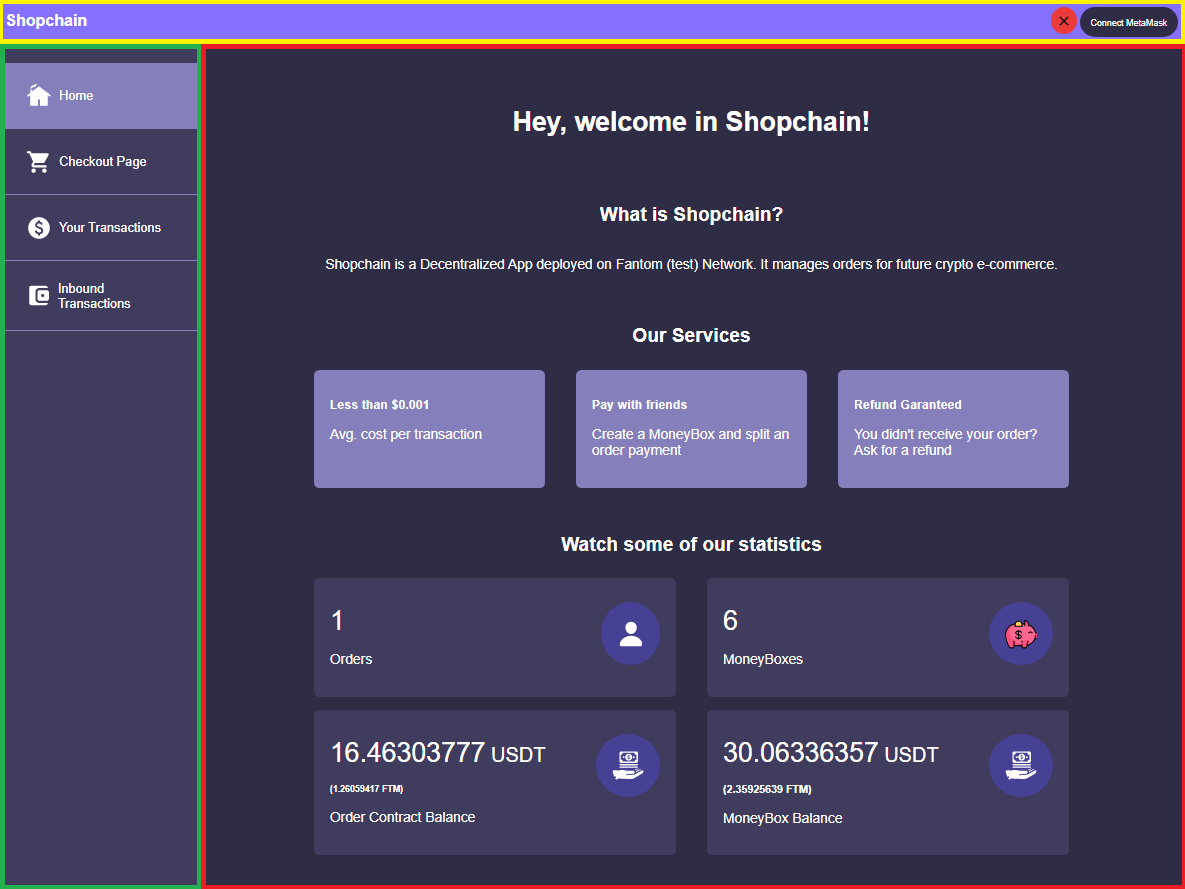
\includegraphics[scale=0.5]{immagini/trePannelli.png}
    \caption{Schema a tre pannelli}
\end{figure}


    \subsection{Navbar} \label{subsection:Navbar}
    La navbar presenta la scritta \projectName{} cliccabile che rimanda direttamente alla home, lo stato della connessione a MetaMask e l'indirizzo del portafoglio connesso.
    \begin{figure}[H]
        \centering
        
\includegraphics[scale=0.5]{immagini/navbar.png}
        \caption{Navbar}
    \end{figure}
    \textbf{}\\
    La prima cosa da fare una volta all'interno del sito è effettuare la connessione a MetaMask. Per farlo è sufficiente cliccare il bottone "Connect MetaMask".\\
    A questo punto si aprirà un popup dell'estensione che chiederà di inserire la password scelta al momento dell'iscrizione.\\
    Una volta inserita la password la connessione sarà stabilita.\\
    Qualora non si fosse connessi a MetaMask, \projectName{} risulterà inutilizzabile nella gran parte delle pagine (praticamente tutte quelle in cui è necessaria l'interazione con lo stesso e, di conseguenza, le pagine figlie.), le quali saranno oscurate da un overlay che richiederà di effettuare la connessione:
    \begin{figure}[H]
        \centering
        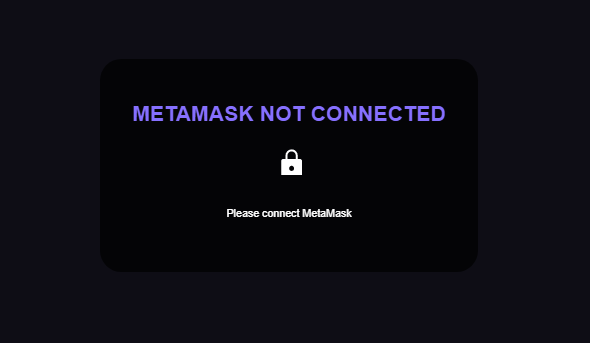
\includegraphics[scale=0.4]{immagini/MetaMaskLayer.png}
        \caption{Overlay "METAMASK NON CONNESSO"}
    \end{figure}
    \textbf{}\\
    Una volta connessi, il proprio indirizzo verrà visualizzato sotto forma di stringa di Emoji e al passaggio del mouse sotto forma di semplice stringa.
    \begin{figure}[H]
        \centering
        
\includegraphics[scale=0.7]{immagini/emoji.png}
        \caption{Indirizzo Emoji e stringa}
    \end{figure}
    \textbf{}\\
    L'icona a sinistra dell'indirizzo del portafoglio segnala appunto lo stato della connessione alla rete Fantom\glo{}.\\
    Posizionandosi sopra l'icona sarà possibile reperire un messaggio relativo allo stato della connessione a MetaMask. Di seguito alcuni esempi:
    \begin{figure}[H]
        \centering
        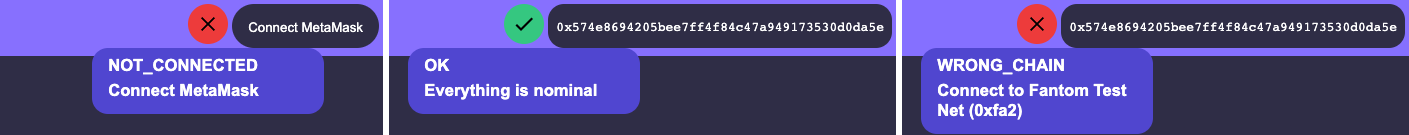
\includegraphics[scale=0.3]{immagini/stateSignal.png}
        \caption{Messaggi di stato della connessione}
    \end{figure}

    \subsection{Menù e Contenuto} \label{subsection:Menu_E_Contenuto}
    Il menù di navigazione presenta le seguenti sezioni:
    \begin{itemize}
        \item \textbf{Home};
        \item \textbf{Checkout Page};
        \item \textbf{Your Transactions};
        \item \textbf{Inbound Transactions};
    \end{itemize}

    Tutte le sezioni sopracitate vengono poi visualizzate all'interno del pannello dei contenuti.

    
        \subsubsection{Home}
        La home di \projectName{} contiene solamente alcune informazioni riguardanti il sito stesso.
        \begin{figure}[H]
            \centering
            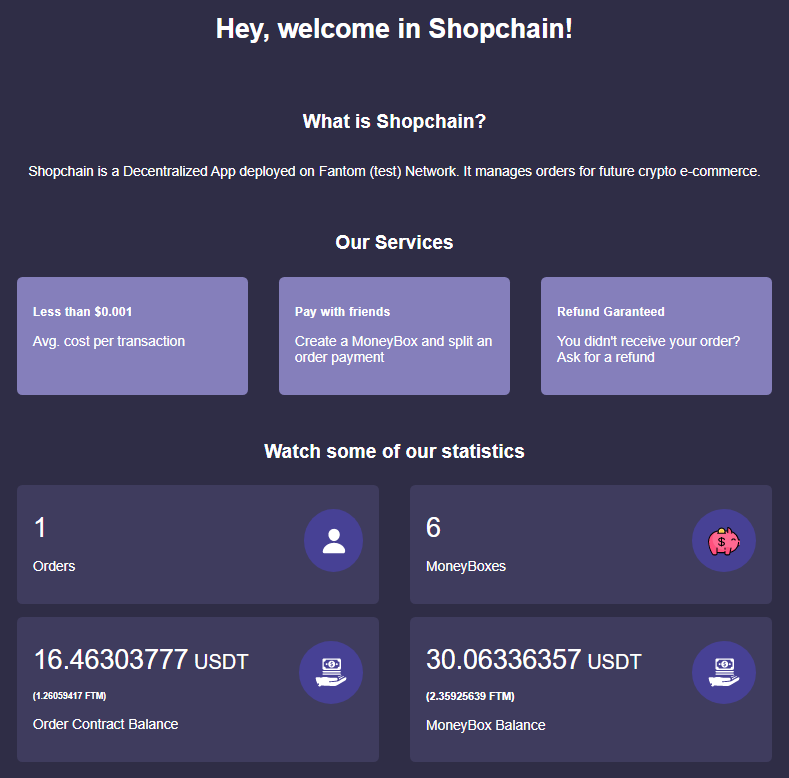
\includegraphics[scale=0.5]{immagini/Home.png}
            \caption{HomePage di \projectName{}}
        \end{figure}
        \textbf{}\\
        Potrebbe risultare interessante dare uno sguardo alle statistiche riguardanti il contratto:
        \begin{figure}[H]
            \centering
            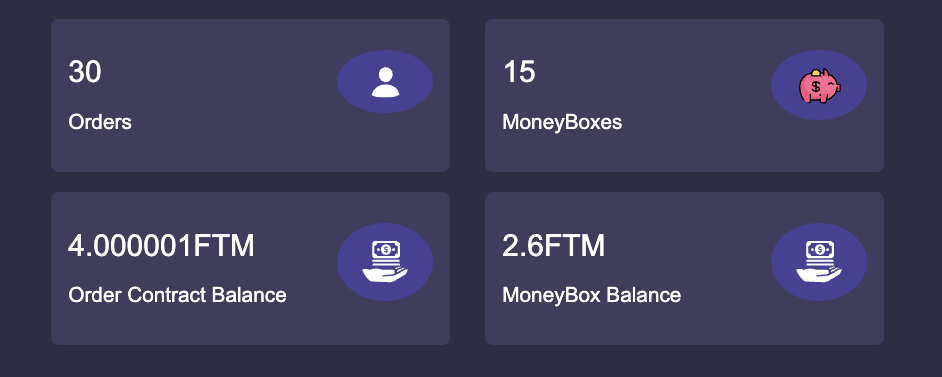
\includegraphics[scale=0.4]{immagini/ContractDetails.png}
            \caption{Statistiche contratto}
        \end{figure}
        \textbf{}\\
        Esse rappresentano gli ordini effettuati su \projectName{} da quando è in funzione e quanto denaro è attualmente depositato all'interno del contratto. Le icone di sinistra raccolgono le informazioni riguardanti gli ordini singoli, mentre quelle di destra riguardano le MoneyBox.
        \subsubsection{Checkout Page} \label{subsection: CheckoutPage}
        Cliccando su Checkout Page, nel menù, verremo reindirizzati alla seguente pagina:
        \begin{figure}[H]
            \centering
            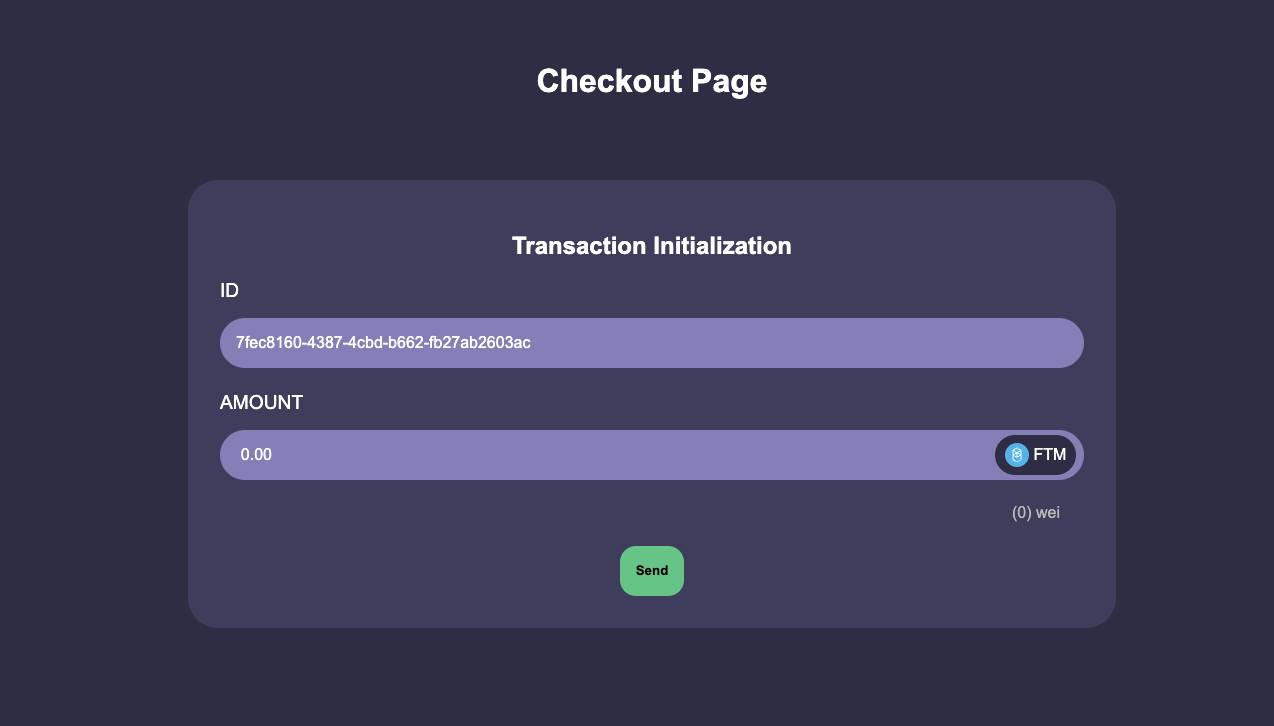
\includegraphics[scale=0.3]{immagini/Checkout/Checkout.png}
            \caption{Checkout Page}
        \end{figure}
        \textbf{}\\
        La pagina di Checkout presenta un form con i campi ID e AMOUNT.\\
        Questa pagina risulta essere esclusivamente dimostrativa in quanto tali dati saranno successivamente reperiti direttamente dall'e-commerce\glo{} e non saranno modificabili né dalla piattaforma né dall'utente.\\
        Allo scopo di mostrare il funzionamento dell'applicativo, poiché il sito non risulta effettivamente collegato a nessun e-commerce\glo{}, è possibile scegliere un ammontare da pagare. \\
        Una volta scelto l'importo sarà sufficiente cliccare il tasto \texttt{"Send"} per proseguire.\\
        Ovviamente per proseguire è necessario inserire un importo superiore a 0. Nel caso in cui questo non dovesse verificarsi verrà segnalato un errore di avviso come segue:
        \begin{figure}[H]
            \centering
            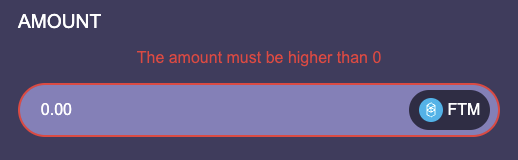
\includegraphics[scale=0.4]{immagini/Checkout/biggerThanZero.png}
            \caption{L'importo deve essere superiore a 0}
        \end{figure}
        A questo punto ci troveremo davanti alla pagina di scelta della modalità del pagamento:
        \begin{figure}[H]
            \centering
            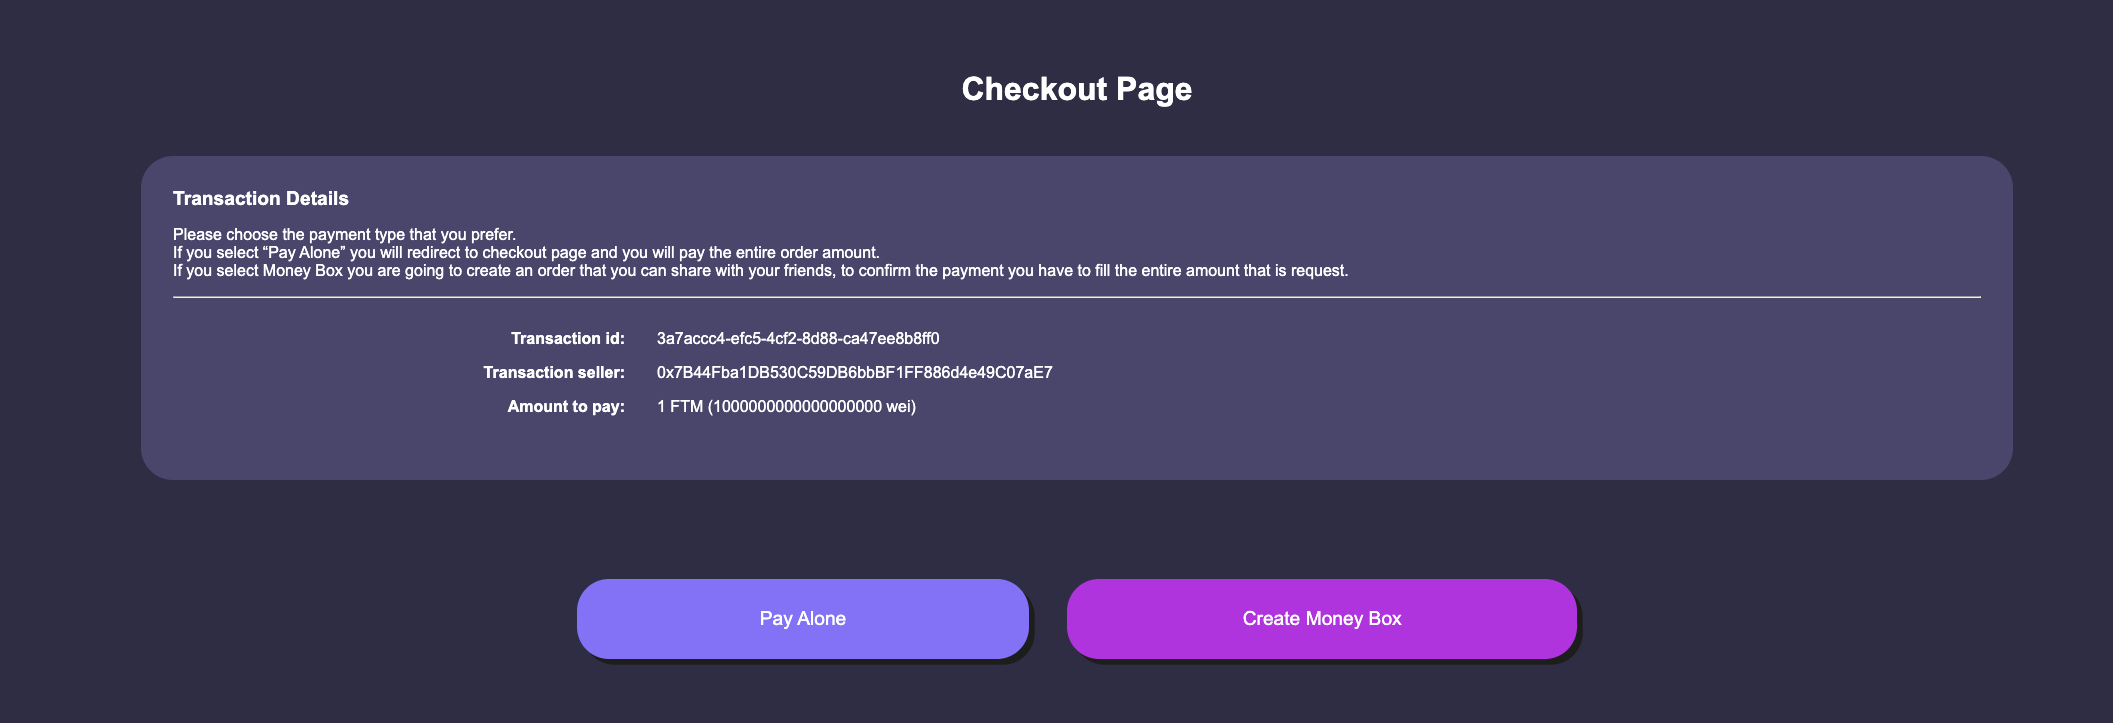
\includegraphics[scale=0.4]{immagini/Checkout/PaymentMode.png}
            \caption{Pagina di scelta modalità di pagamento}
        \end{figure}
        \textbf{}\\
        Nel particolare in questa pagina è possibile trovare il riassunto della transazione con  il suo identificativo, l'indirizzo del venditore a cui stiamo mandando il denaro e l'importo totale da pagare.\\\\
        Successivamente analizzeremo le differenze e i dettagli delle due modalità di pagamento.
            \paragraph{Pagamento Singolo}
            \begin{figure}[H]
                \centering
                
\includegraphics[scale=0.3]{immagini/Checkout/PayAlone.png}
                \caption{Tasto scelta modalità pagamento singolo}
            \end{figure}
            Cliccando il tasto \texttt{"Pay Alone"} verrà aperto un popup dall'estensione MetaMask con i dettagli del pagamento e la possibilità di confermare o annullare il pagamento. Un overlay di caricamento apparirà nella pagina \projectName{} fintantoché la transazione non sarà conclusa come mostrato nella figura seguente:
            \begin{figure}[H]
                \centering
                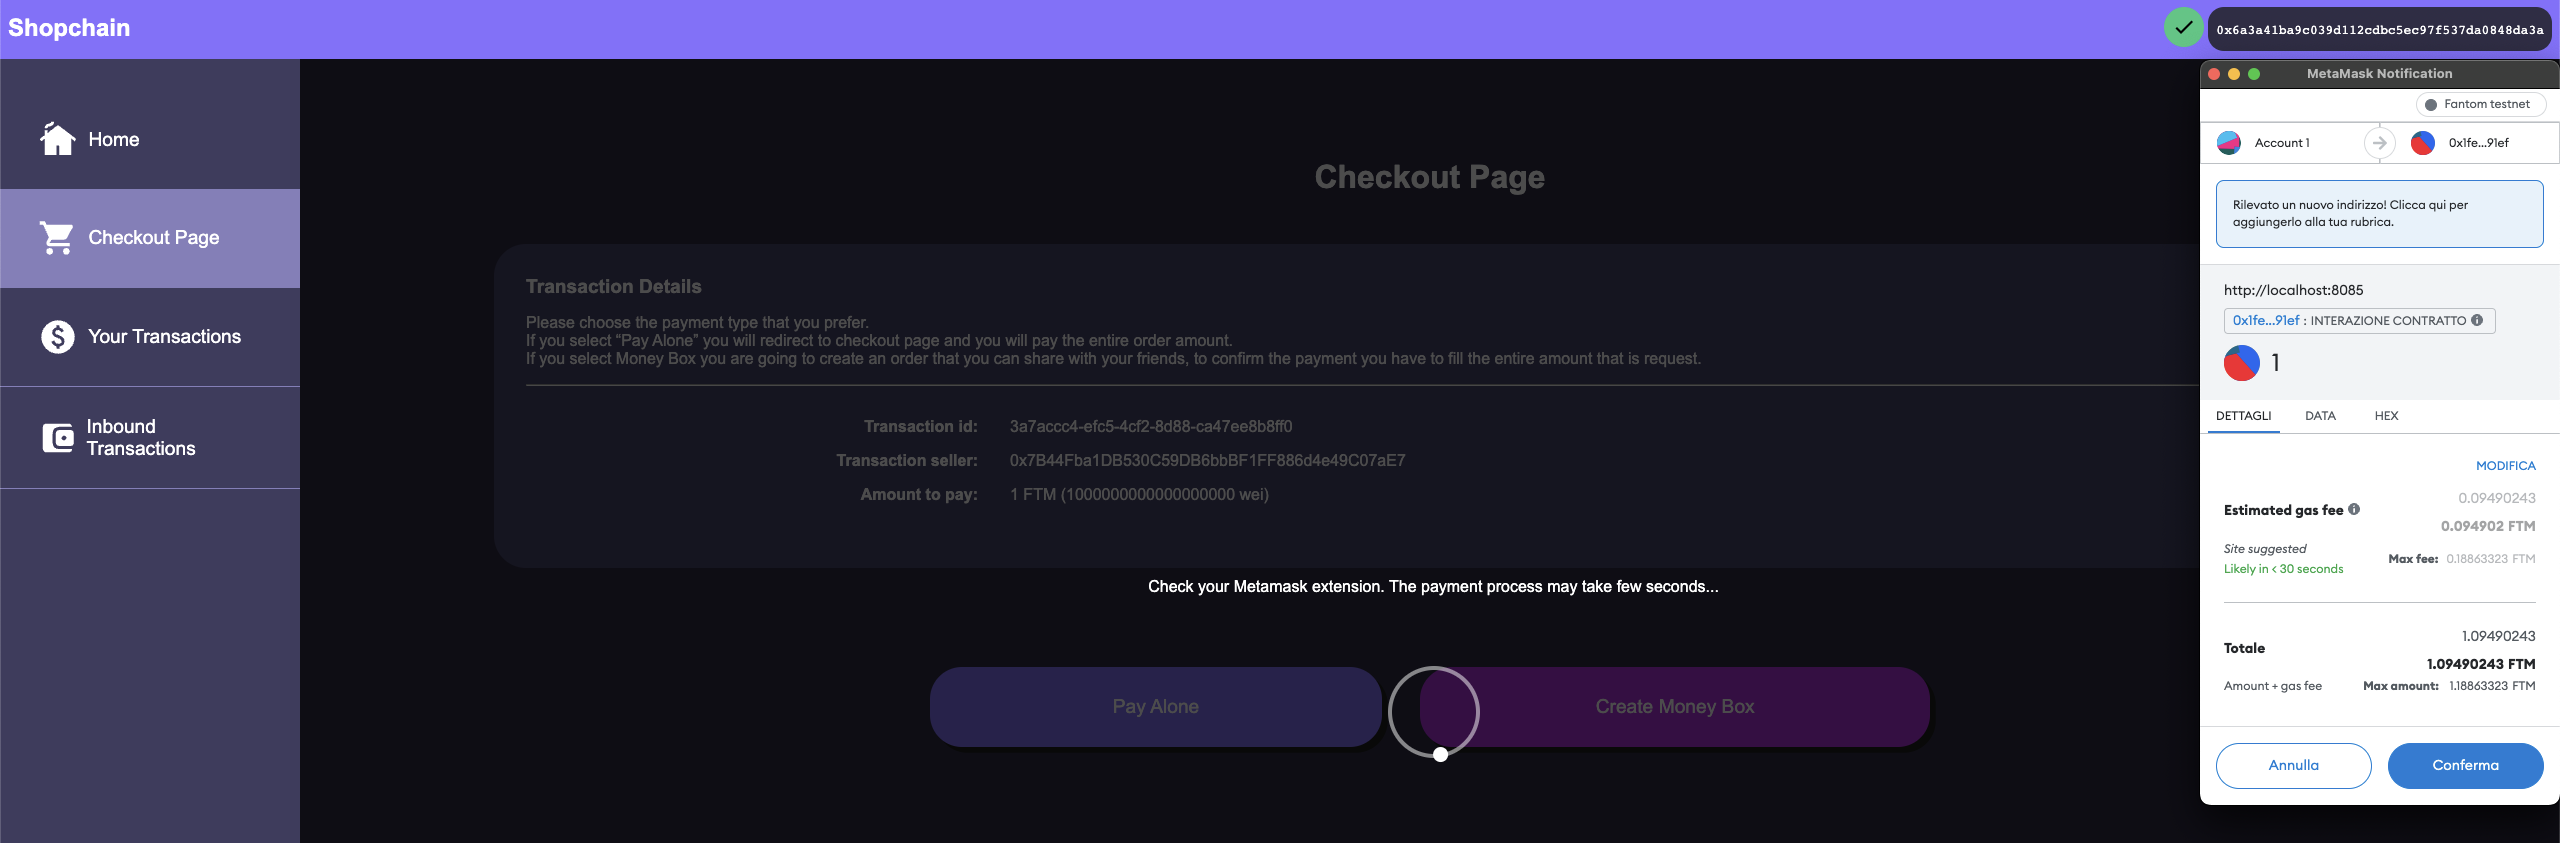
\includegraphics[scale=0.4]{immagini/Checkout/SinglePaymentLayer.png}
                \caption{Fase di pagamento singolo}
            \end{figure}
            \textbf{}\\
            Una volta che la transazione sarà stata registrata (in genere pochi secondi dopo averla confermata), si verrà reindirizzati a una pagina che conferma che la transazione è avvenuta correttamente:
            \begin{figure}[H]
                \centering
                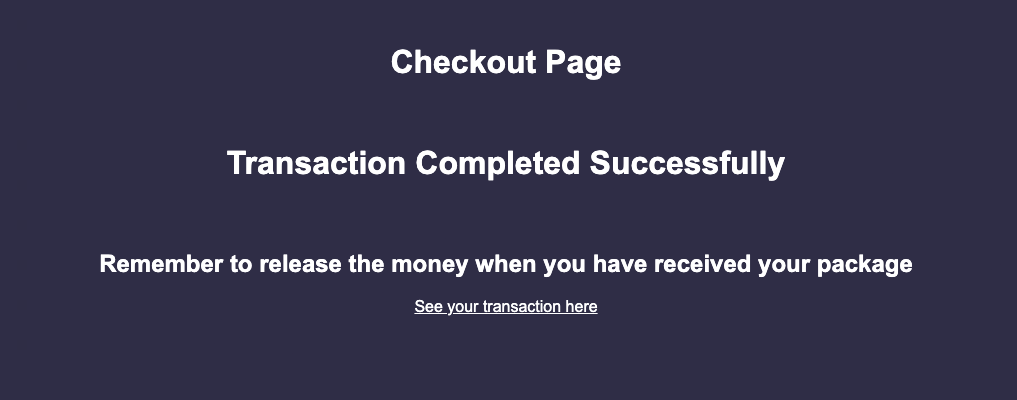
\includegraphics[scale=0.3]{immagini/Checkout/PayAloneTransactionSuccess.png}
                \caption{Transazione avvenuta con successo}
            \end{figure}
            \textbf{}\\
            Da qui sarà possibile visualizzare il dettaglio della transazione semplicemente cliccando il link \texttt{"See your transaction here"} attraverso il quale si verrà reindirizzati alla pagina mostrata di seguito:
            \begin{figure}[H]
                \centering
                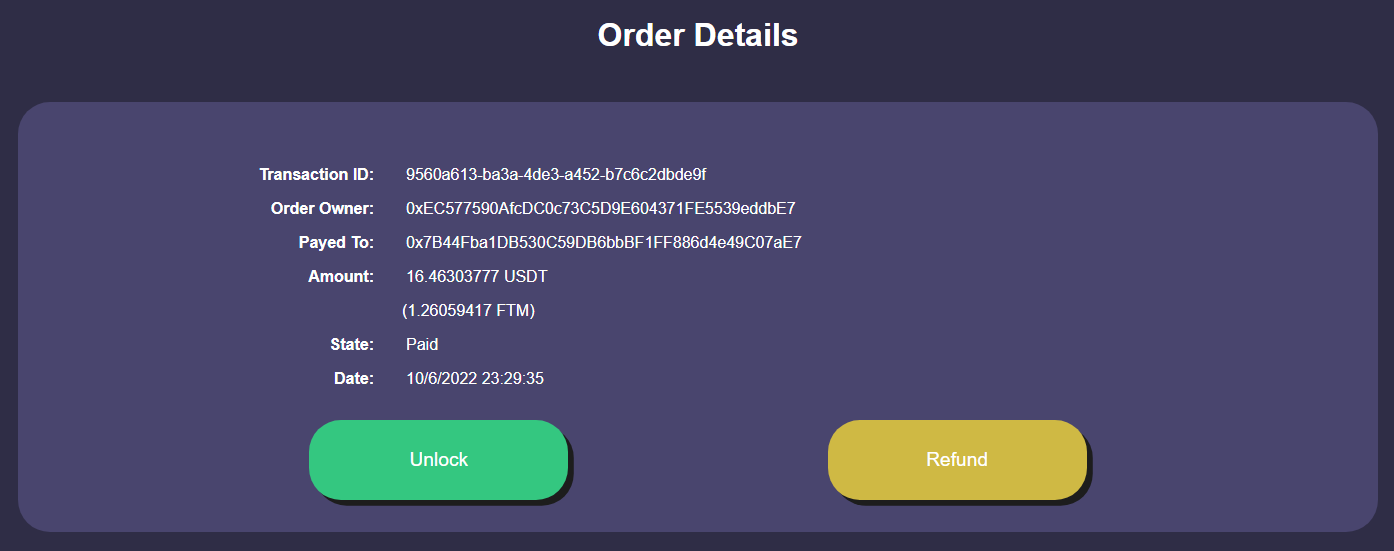
\includegraphics[scale=0.4]{immagini/Checkout/SinglePaymentDetails.png}
                \caption{Dettaglio transazione singola}
            \end{figure}
            \textbf{}\\
            Da qui sarà quindi possibile sbloccare il denaro attraverso un codice di sblocco (una volta ricevuto l'ordine) o chiedere il rimborso (qualora l'ordine non venga mai recapitato) mediante gli appositi bottoni.
            \paragraph{Pagamento MoneyBox}
            \begin{figure}[H]
                \centering
                
\includegraphics[scale=0.3]{immagini/Checkout/CreateMoneyBox.png}
                \caption{Tasto scelta modalità pagamento MoneyBox}
            \end{figure}
            Cliccando il tasto \texttt{"Create MoneyBox"} verrà scelta la modalità di pagamento MoneyBox e la pagina mostrata sarà la seguente:
            \begin{figure}[H]
                \centering
                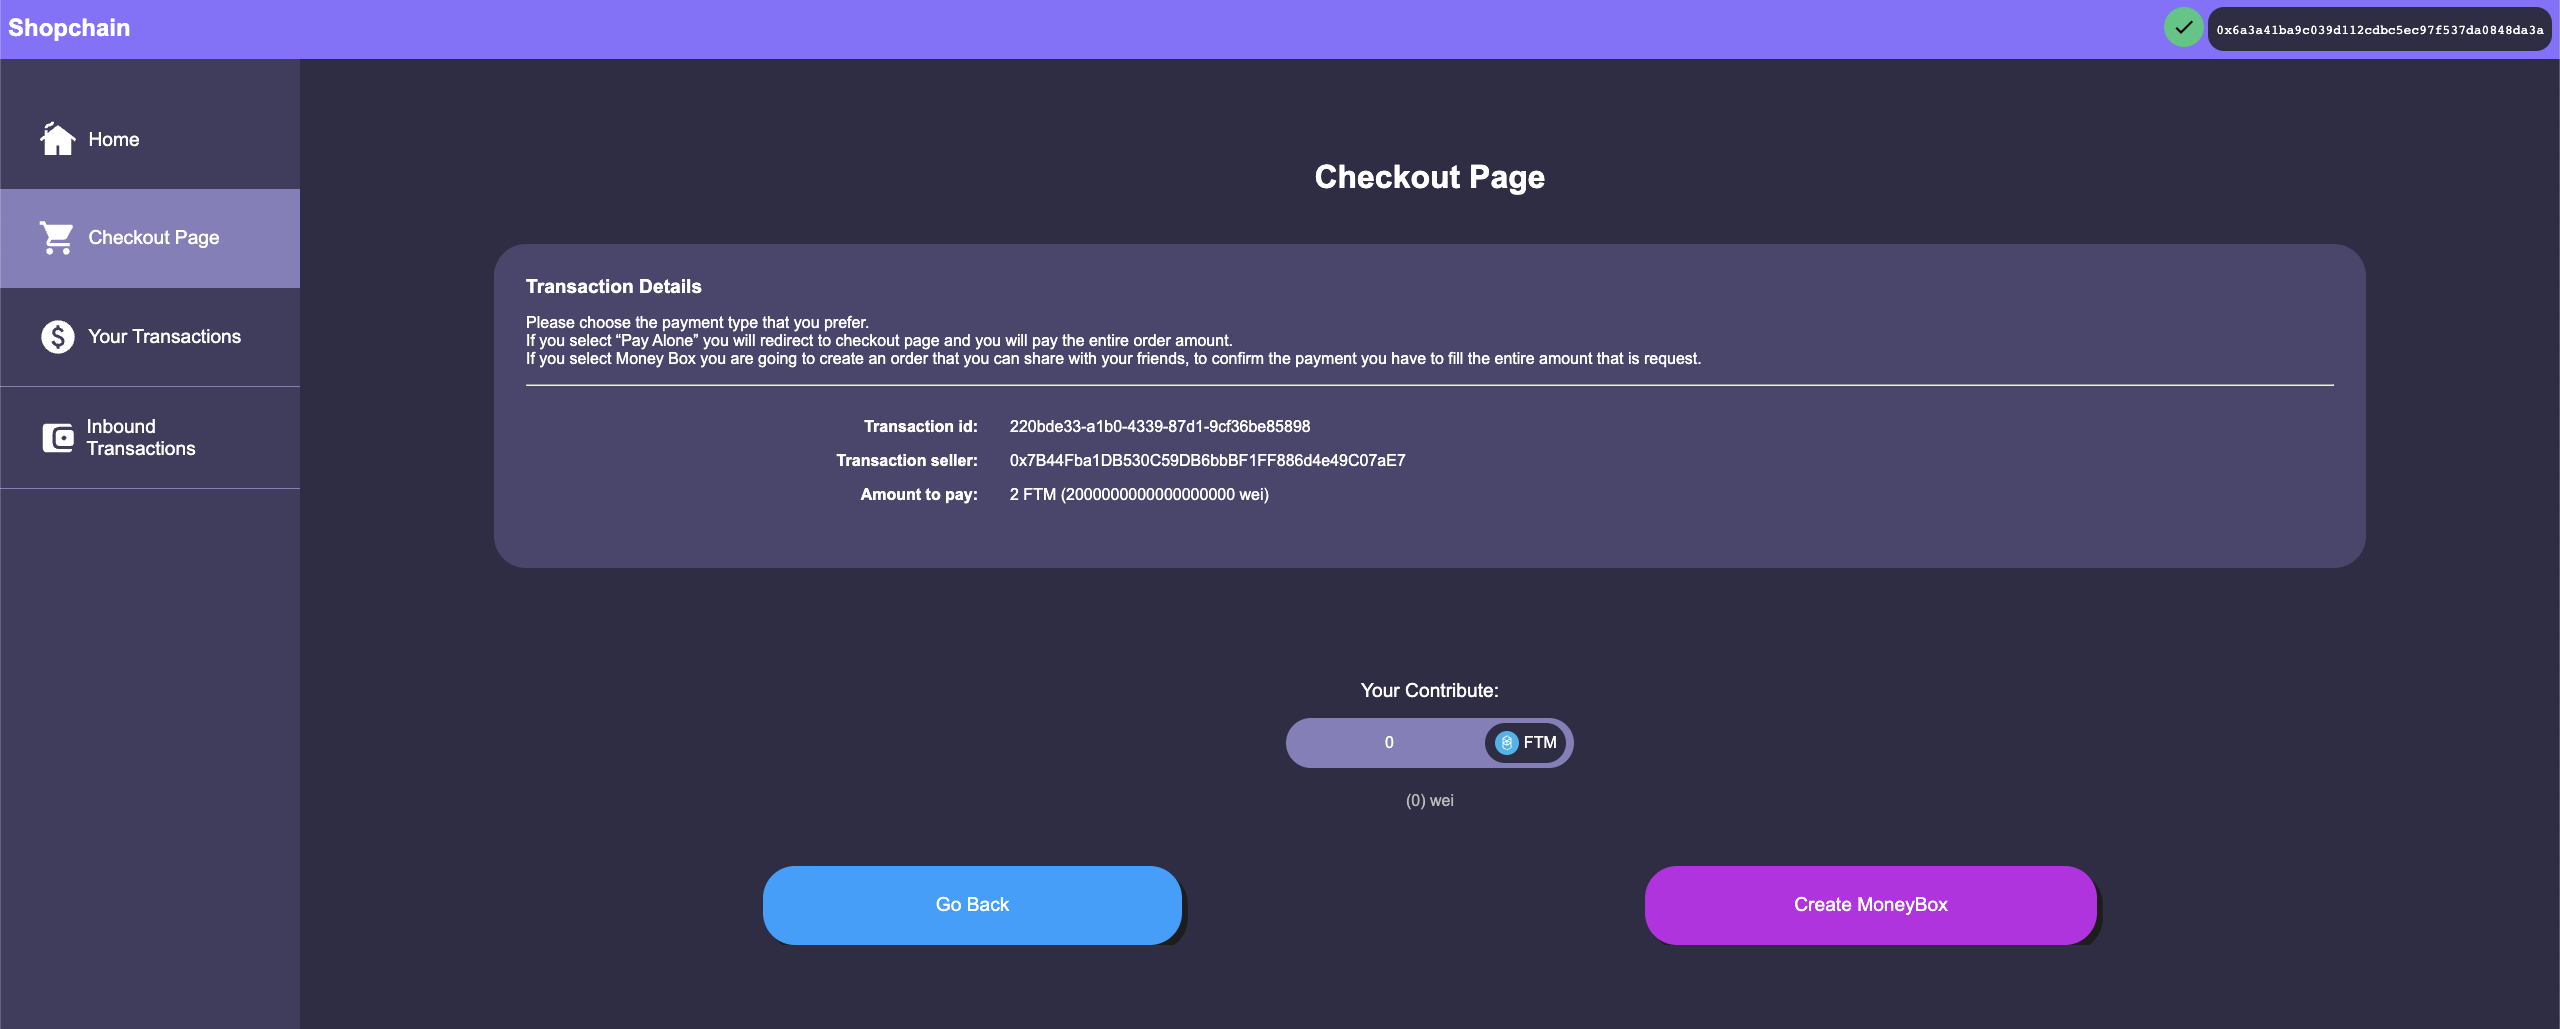
\includegraphics[scale=0.4]{immagini/Checkout/MoneyBoxCheckout.png}
                \caption{Pagina Checkout MoneyBox}
            \end{figure}
            \textbf{}\\
            Analizzando la pagina è possibile vedere il dettaglio della transazione, un box per inserire l'eventuale proprio contributo fin dalla creazione e i tasti \texttt{"Go Back"} e \texttt{"Create MoneyBox"}.\\\\
            Per inserire un contributo sarà necessario inserire l'importo all'interno del box come mostrato di seguito:
            \begin{figure}[H]
                \centering
                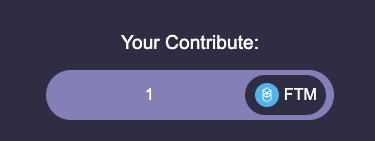
\includegraphics[scale=0.4]{immagini/Checkout/InitialContribute.png}
                \caption{Contributo MoneyBox in fase di creazione}
            \end{figure}
            \textbf{}\\
            e in seguito cliccare il bottone \texttt{"Create MoneyBox"}.\\\\
            \textbf{N.B.} \textit{Se si ha intenzione di versare una quota, è consigliato farlo al momento della creazione della MoneyBox, così da pagare una sola volta le gasfee necessarie all'interazione con il contratto.}\\\\
            A questo punto verrà aperto un popup dall'estensione MetaMask con i dettagli del pagamento e la possibilità di confermare o annullare il pagamento. Un overlay di caricamento apparirà nella pagina \projectName{} fintantoché la transazione non sarà conclusa, come mostrato nella figura seguente:
            \begin{figure}[H]
                \centering
                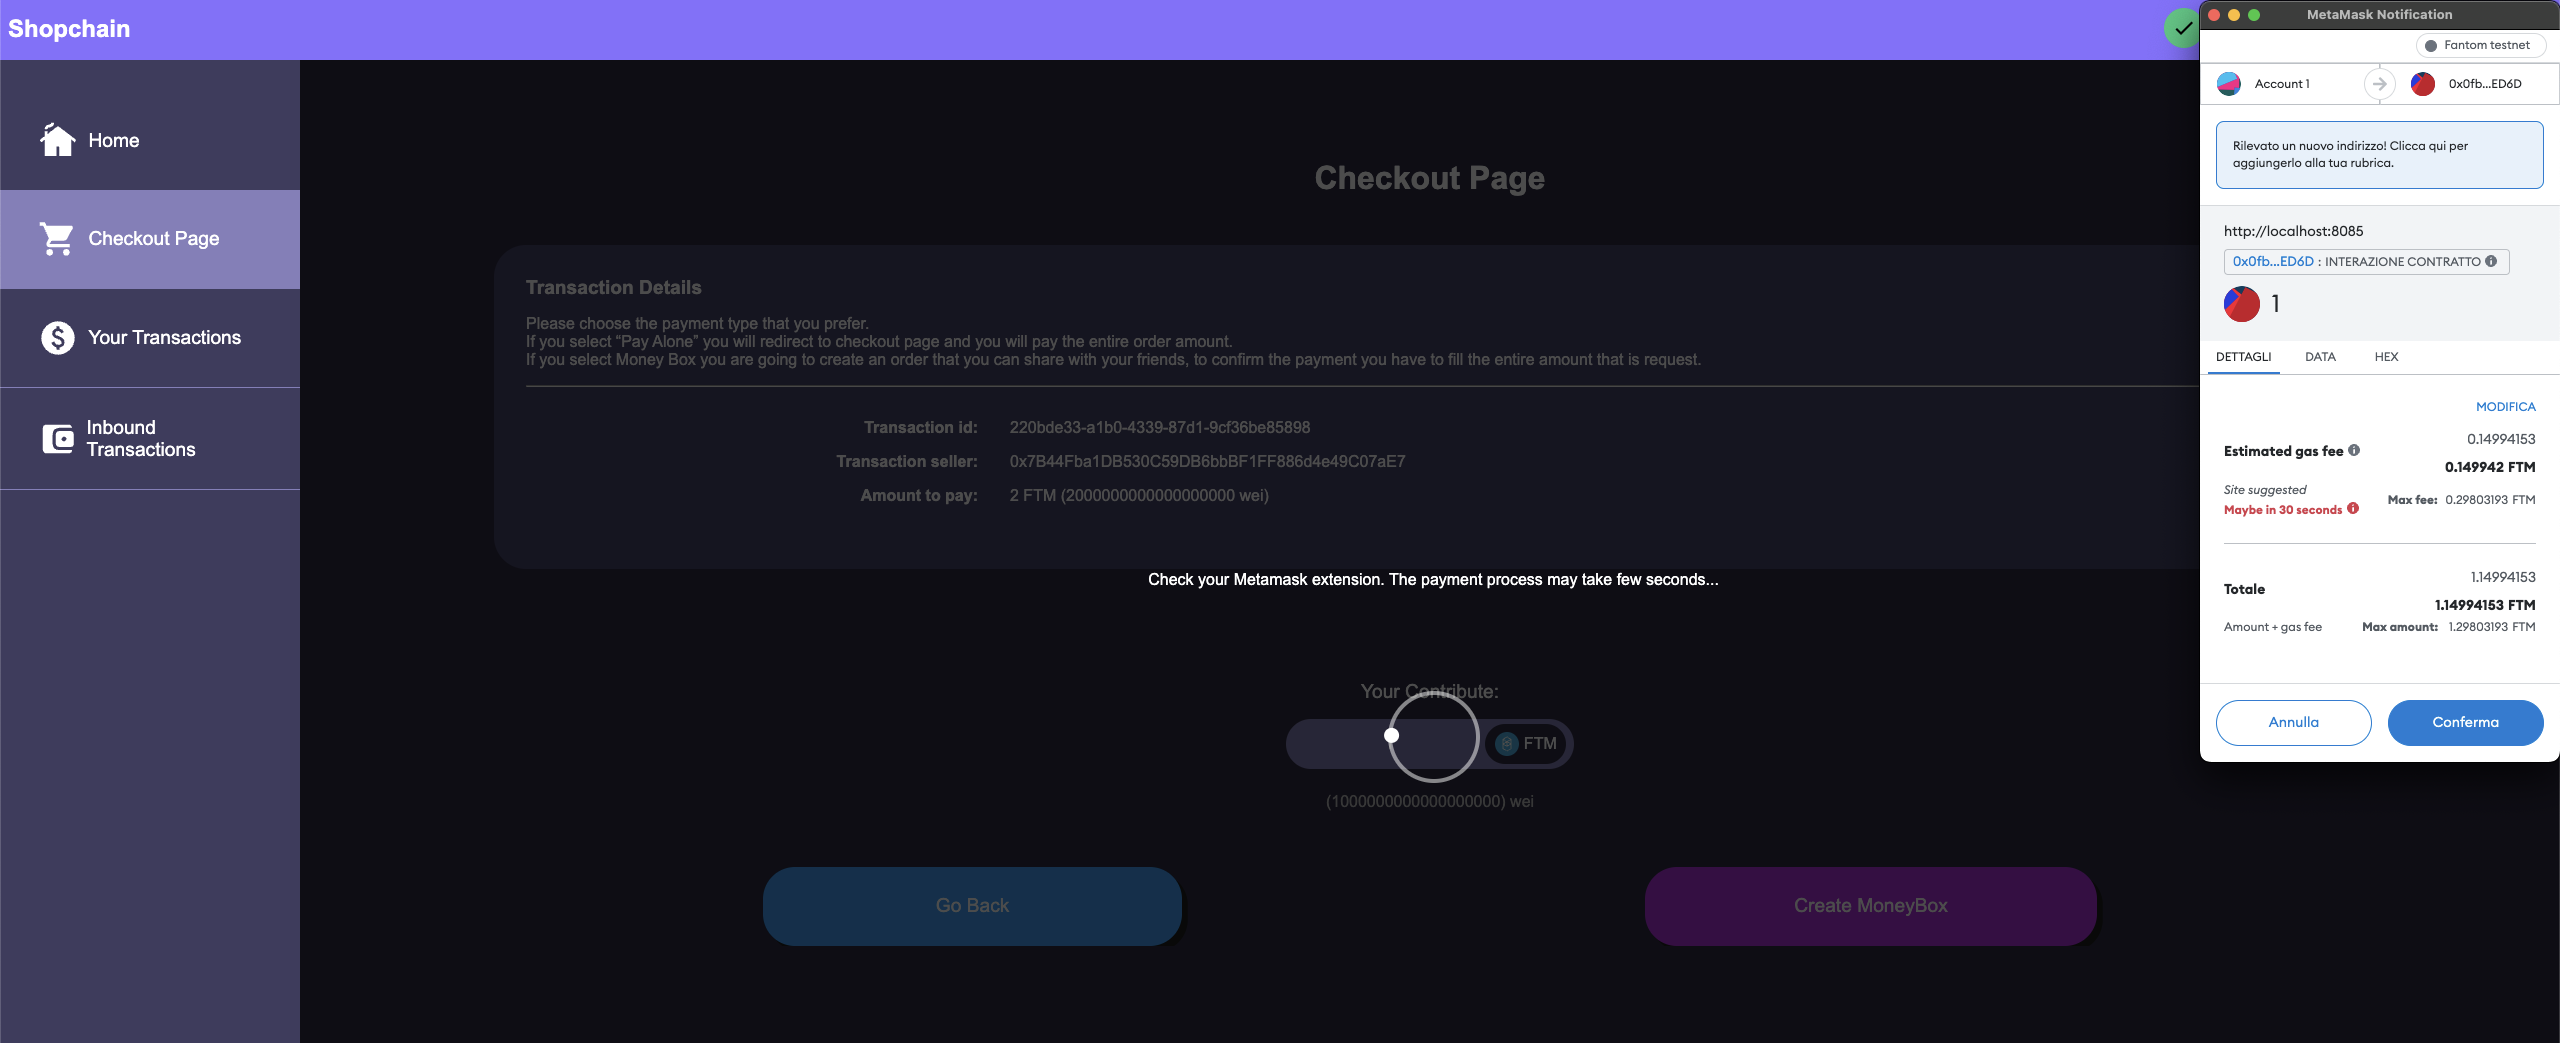
\includegraphics[scale=0.15]{immagini/Checkout/MoneyBoxLayer.png}
                \caption{Fase di pagamento MoneyBox}
            \end{figure}
            \textbf{}\\
            Una volta che la transazione sarà stata registrata (in genere pochi secondi dopo averla confermata), si verrà reindirizzati a una pagina che conferma che la transazione è avvenuta correttamente:
            \begin{figure}[H]
                \centering
                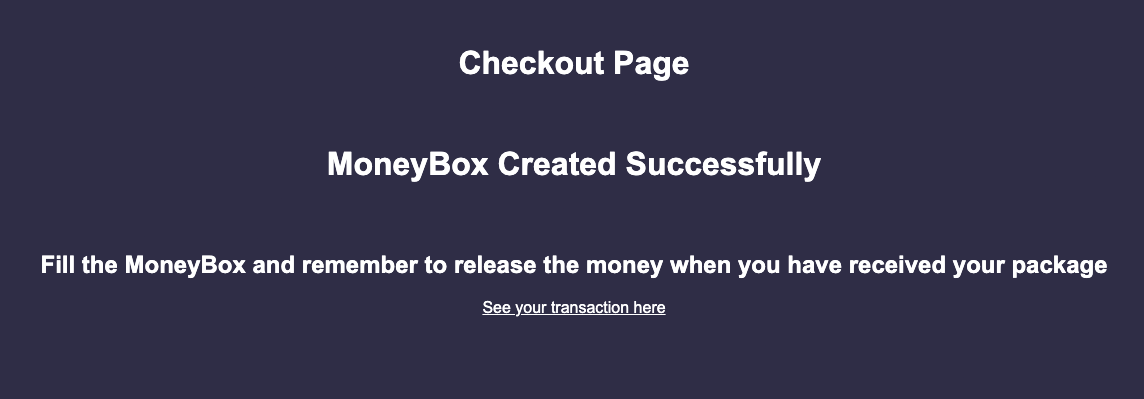
\includegraphics[scale=0.3]{immagini/Checkout/MoneyBoxTransactionSuccess.png}
                \caption{creazione MoneyBox avvenuta con successo}
            \end{figure}
            \textbf{}\\
            Da qui sarà possibile visualizzare il dettaglio della transazione semplicemente cliccando il link \texttt{"See your transaction here"} attraverso il quale si verrà reindirizzati alla pagina mostrata di seguito:
            \begin{figure}[H]
                \centering
                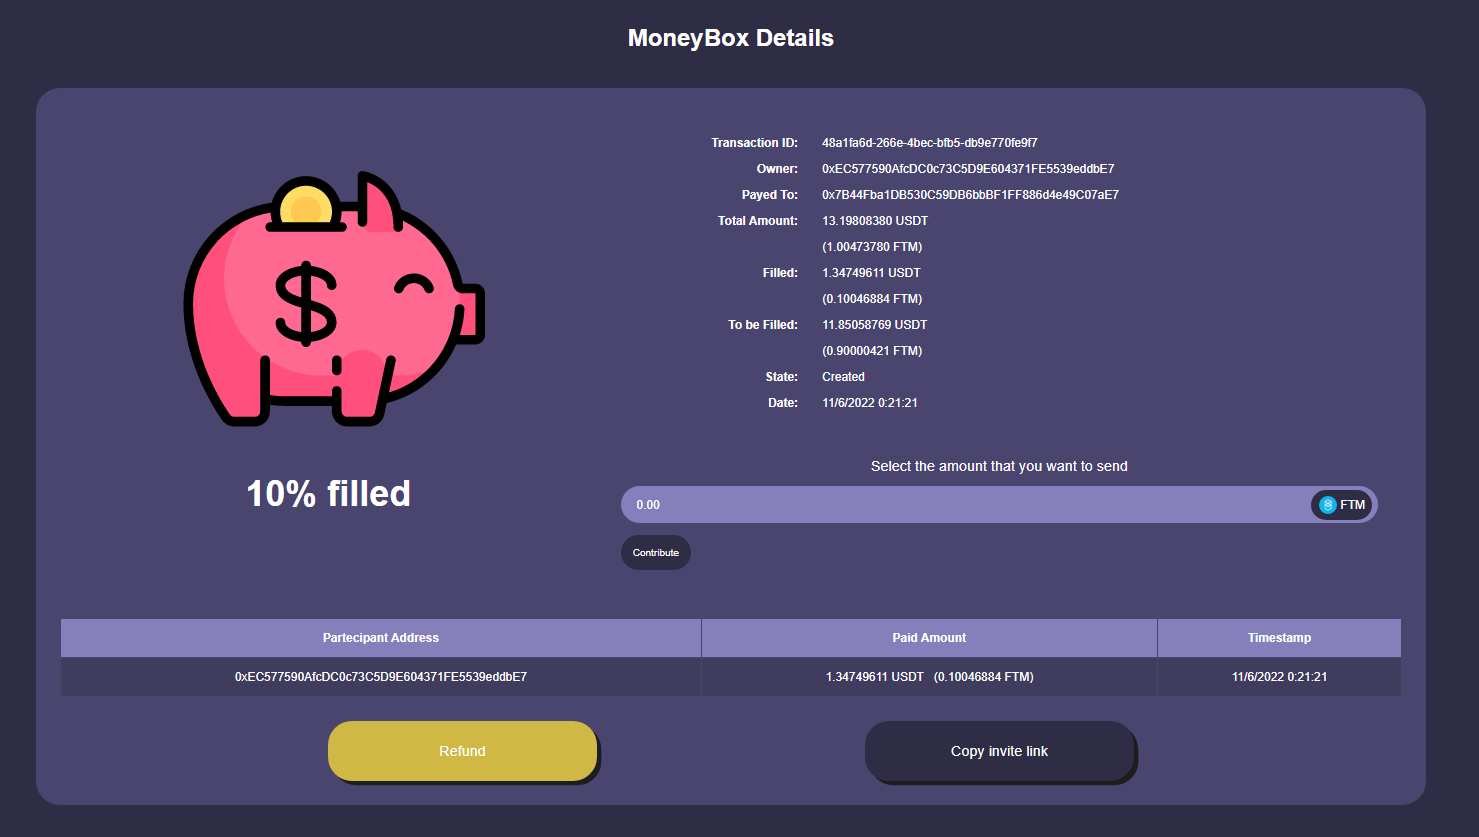
\includegraphics[scale=0.4]{immagini/Checkout/MoneyBoxDetails.png}
                \caption{Dettaglio transazione MoneyBox}
            \end{figure}
            \textbf{}\\
            Da qui sarà quindi possibile copiare il link di invito cliccando il bottone \texttt{"Copy invite link"}, da condividere con i contribuenti alla MoneyBox, o chiedere il rimborso qualora la MoneyBox debba essere annullata o l'ordine non venga mai recapitato.\\
            All'interno della pagina è inoltre possibile notare altre informazioni quali la percentuale di riempimento della MoneyBox, un box per contribuire alla MoneyBox e una tabella con il dettaglio delle transazioni dei contribuenti.\\
            Per condividere la MoneyBox con gli altri contribuenti sarà sufficiente condividere il link di invito precedentemente descritto e che l'utente contribuente disponga di tutti i requisiti citati fino a questo punto.\\
            Quando la MoneyBox sarà completamente riempita il suo stato passerà da \texttt{"Created"} a \texttt{"Paid"} e comparirà l'apposito bottone che permetterà di effettuare lo sblocco del denaro al wallet del venditore.\\\\ 
            \textbf{N.B.} \textit{Solo l'utente che ha creato la MoneyBox potrà effettuare lo sblocco.}\\\\
            Le immagini a seguire mostrano in dettaglio il box per inserire il proprio contributo, la tabella dei contribuenti e un esempio di come la pagina si trasforma quando la MoneyBox passa allo stato \texttt{"Paid"}:
            \begin{figure}[H]
                \centering
                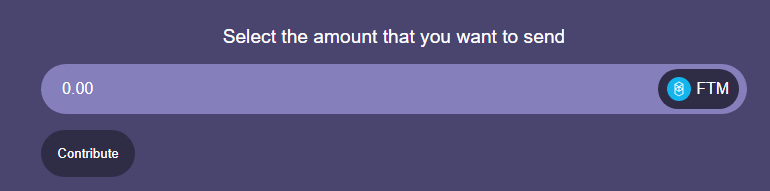
\includegraphics[scale=0.3]{immagini/Checkout/Contribute.png} 
                \caption{Box per inserire il proprio contributo alla MoneyBox}
            \end{figure}
            \begin{figure}[H]
                \centering
                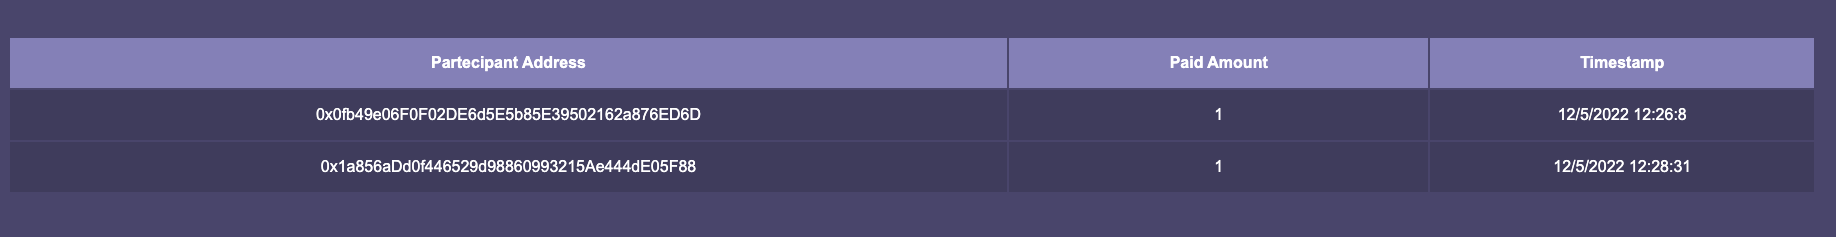
\includegraphics[scale=0.25]{immagini/Checkout/ContributionsTable.png} 
                \caption{Tabella dettaglio contribuenti}
            \end{figure}
            \begin{figure}[H]
                \centering
                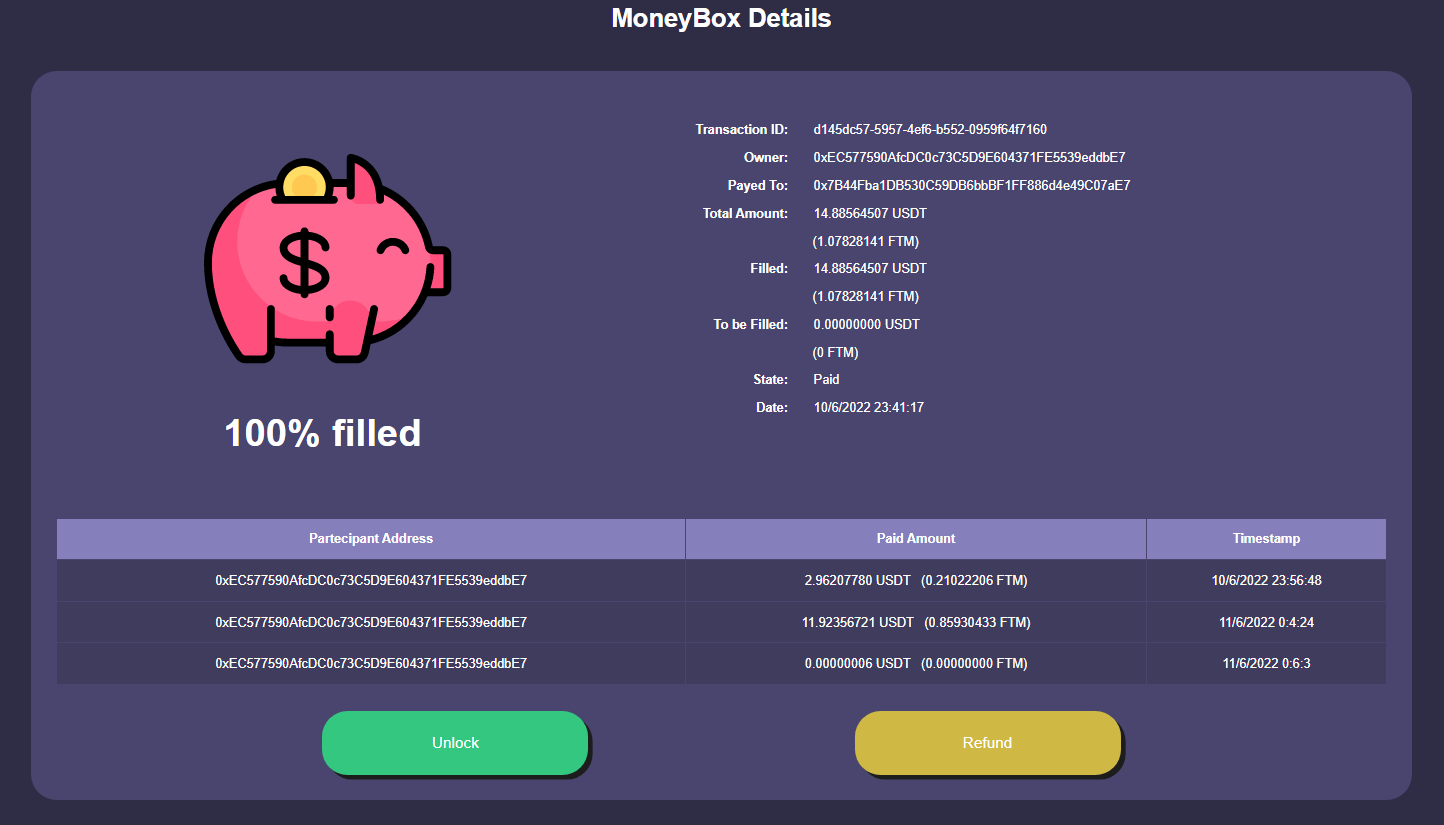
\includegraphics[scale=0.4]{immagini/Checkout/FilledMoneyBox.png} 
                \caption{Dettaglio MoneyBox in stato \texttt{"Paid"}}
            \end{figure}
            \textbf{}\\
            Da quest'ultima figura in particolare è possibile notare la comparsa del bottone di sblocco e la scomparsa del box per contribuire alla MoneyBox poiché, in quanto già piena, non è più possibile inserire denaro al suo interno.\\\\
            Da qui sarà quindi possibile sbloccare il denaro attraverso un codice di sblocco (una volta ricevuto l'ordine) o chiedere il rimborso (qualora l'ordine non venga mai recapitato) mediante gli appositi bottoni.
            \subsubsection{Sblocco e Rimborso}
        Sia nel caso di \texttt{sblocco} che nel caso di \texttt{rimborso}, al click dell'apposito bottone si aprirà un popup in quanto quella che si compie in questa fase è un'operazione irreversibile e dunque considerata sensibile.\\\\
        Nel caso di \textbf{sblocco} verrà mostrato un popup che mostrerà il codice di sblocco e un'input box nella quale replicare tale codice con l'aggiunta di due tasti per la conferma dell'inserimento del codice o la chiusura del popup stesso:
        \begin{figure}[H]
            \centering
            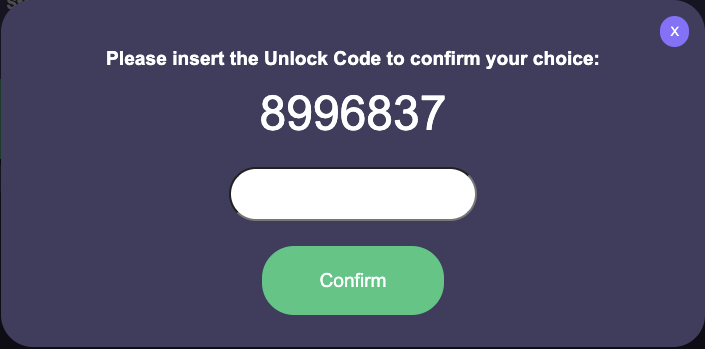
\includegraphics[scale=0.3]{immagini/Checkout/UnlockPopUp.png} 
            \caption{Popup di sblocco}
        \end{figure}
        \textbf{}\\
        Nel caso di \textbf{rimborso} verrà mostrato un semplice popup di conferma così da assicurare una scelta consapevole.
        \begin{figure}[H]
            \centering
            \includegraphics[scale=0.3]{immagini/Checkout/RefundPopUp.png} 
            \caption{Popup di rimborso}
        \end{figure}
        \subsubsection{Transazioni}
        In questa sezione verranno approfondite le sezioni \texttt{"Your Transactions"} e \texttt{"Inbound Transactions"} del menù di navigazione.\\
        Tali sezioni vengono affrontate insieme in quanto molto simili tra di loro.\\
        In particolare:
        \begin{itemize}
            \item \textbf{Your Transactions}: L'utente acquirente può trovare in questa sezione l'elenco dei pagamenti e dei contributi MoneyBox effettuati con \projectName{};
            \item \textbf{Inbound Transactions}: L'utente venditore può trovare in questa sezione l'elenco dei pagamenti in entrata da \projectName{}.
        \end{itemize}
        \paragraph{Your Transactions}
        La pagina delle transazioni in uscita, "Your Transactions", è divisa in due sezioni:
        \begin{itemize}
            \item Your Transactions: in questa sezione sono riportati gli ordini \textbf{creati} dall'utente, siano essi di tipo Single Payment (ordine singolo) o MoneyBox;
            \item Your Contributions: in questa sezione sono riportati gli ordini di tipo MoneyBox a cui l'utente ha contribuito.
        \end{itemize}
        \begin{figure}[H]
        \centering
        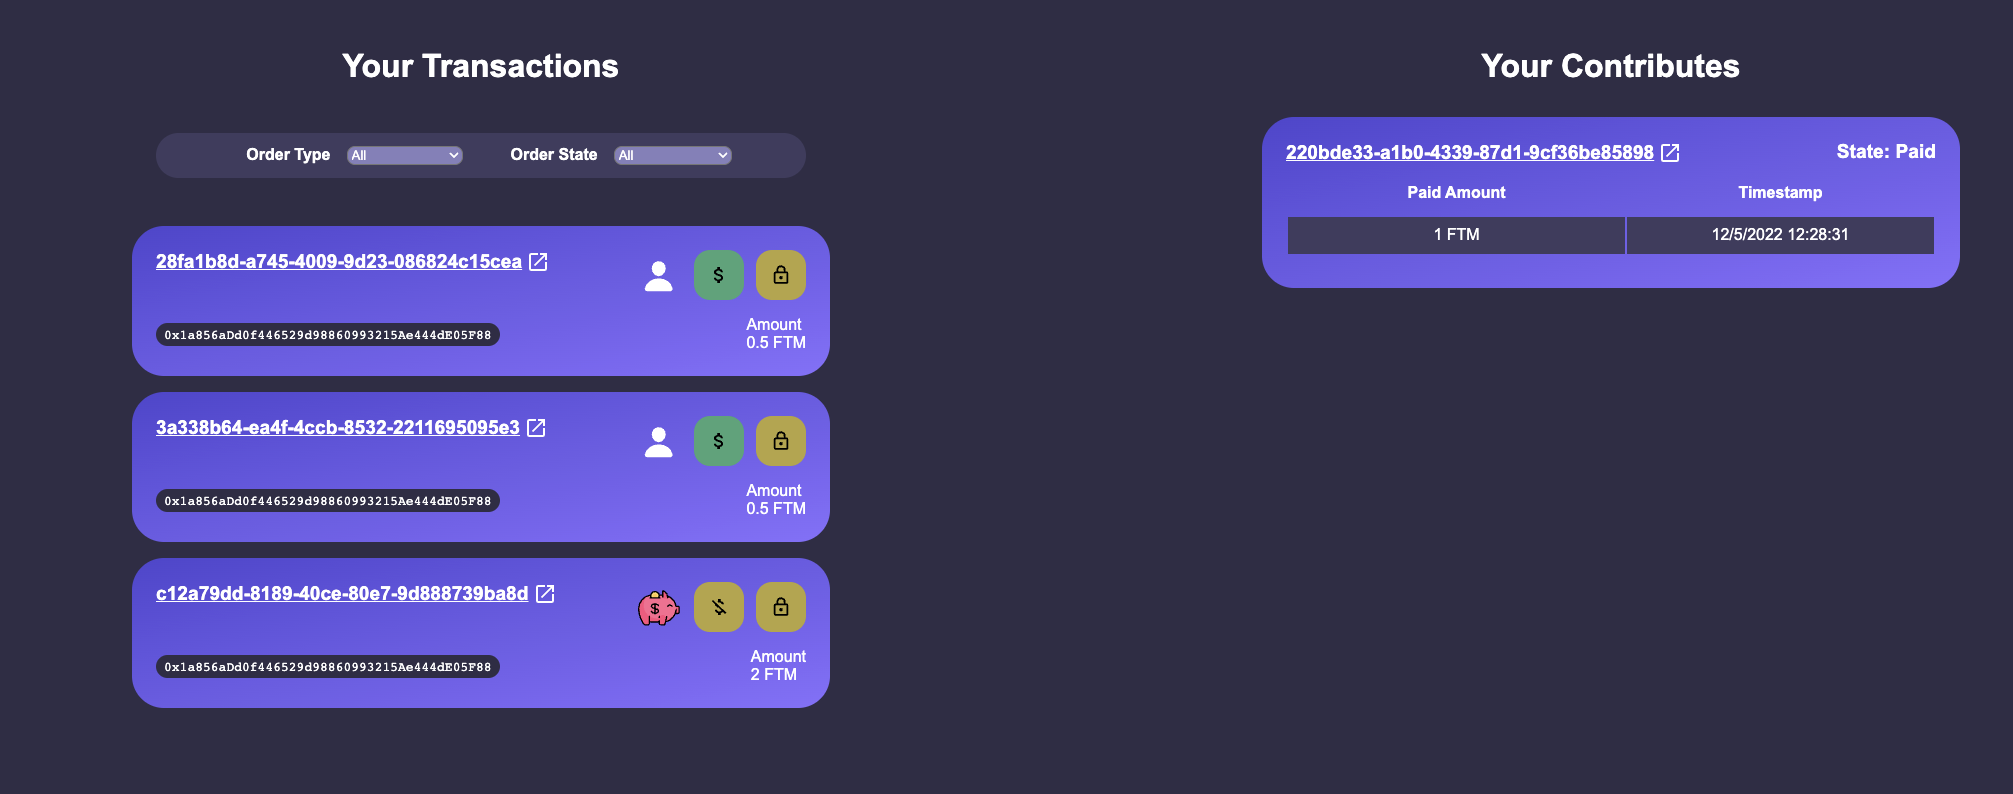
\includegraphics[scale=0.4]{immagini/Transaction/YourTransaction.png}
        \caption{Pagina Your Transactions}
        \end{figure}
        \paragraph{Inbound Transactions}
        La pagina delle transazioni in entrata, "Inbound Transactions", mostra la sezione con le transazioni in entrata verso il wallet dell'utente venditore.\\\\
        \textbf{N.B.} \textit{L'utente venditore potrà vedere esclusivamente le transazioni già pagate.}\\
        \begin{figure}[H]
            \centering
            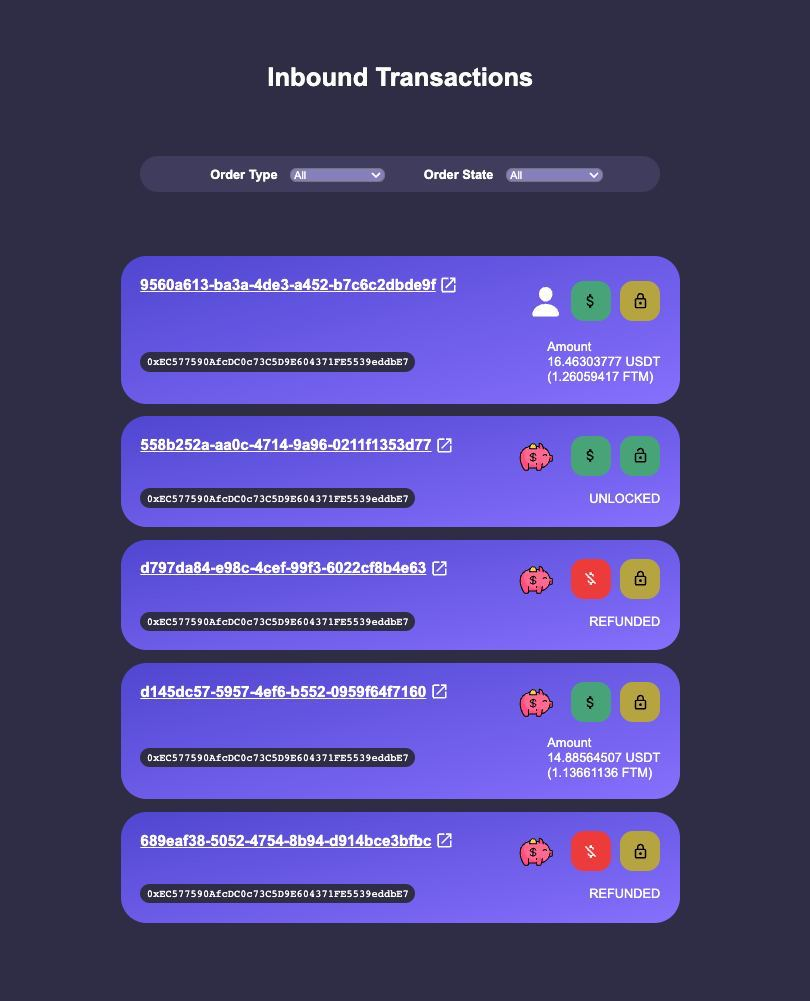
\includegraphics[scale=0.3]{immagini/Transaction/inboundTransactions.png}
            \caption{Pagina Inbound Transactions}
        \end{figure}
        \paragraph{Filtri nelle pagine Transactions}
        Come si può notare dalle immagini precedenti, entrambe le pagine presentano una sezione con menù a tendina.\\
        Tale sezione serve a filtrare gli ordini in base al loro tipo e al loro stato.\\
        In particolare:
        \begin{itemize}
            \item il \textbf{tipo} può assumere i seguenti valori:
            \begin{itemize}
                \item \textbf{All}: Seleziona tutti gli ordini;
                \item \textbf{Single Payment}: Seleziona solo gli ordini di tipo Single Payment;
                \item \textbf{MoneyBox}: Seleziona solo gli ordini di tipo MoneyBox.
            \end{itemize}
            \begin{figure}[H]
                \centering
                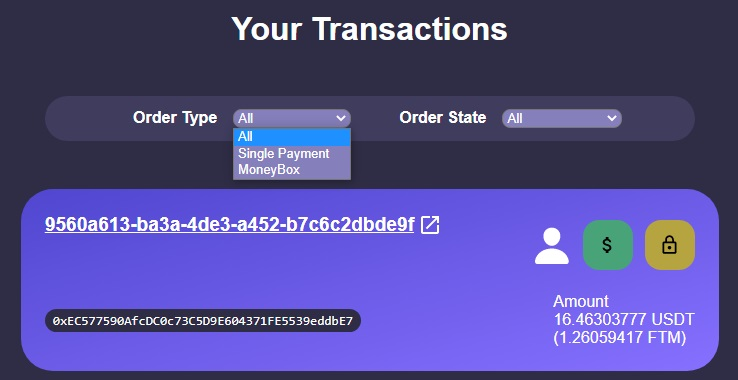
\includegraphics[scale=0.4]{immagini/Transaction/ordertype.jpg}
            \caption{Filtro per la scelta del tipo dell'ordine}
            \end{figure}
            \item Lo \textbf{Stato} può assumere i seguenti valori:
            \begin{itemize}
                \item \textbf{All}: Seleziona tutti gli ordini;
                \item \textbf{To Pay}: Seleziona solo gli ordini che non sono ancora stati pagati;
                \item \textbf{Payd but locked}: Seleziona solo gli ordini in stato "Paid" (che non sono ancora stati sbloccati);
                \item \textbf{Unlocked}: Seleziona solo gli ordini in stato "Unlocked" (che sono state sbloccate);
                \item \textbf{Refunded}: Seleziona solo gli ordini in stato "Refunded" (che sono state rimborsate).
            \end{itemize}
            \begin{figure}[H]
                \centering
                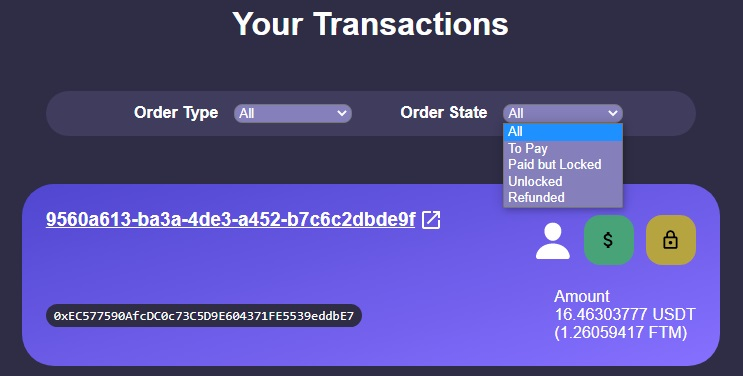
\includegraphics[scale=0.4]{immagini/Transaction/orderstate.jpg}
                \caption{Filtro per la scelta dello stato dell'ordine}
            \end{figure}
        \end{itemize}
        
        \paragraph{Scheda della transazione}
        In questa sezione analizzeremo in maniera dettagliata la scheda di una singola transazione presente all'interno delle pagine riguardanti le transazioni.
        Prendiamo come esempio le schede presenti nell'immagine seguente:
        \begin{figure}[H]
            \centering
            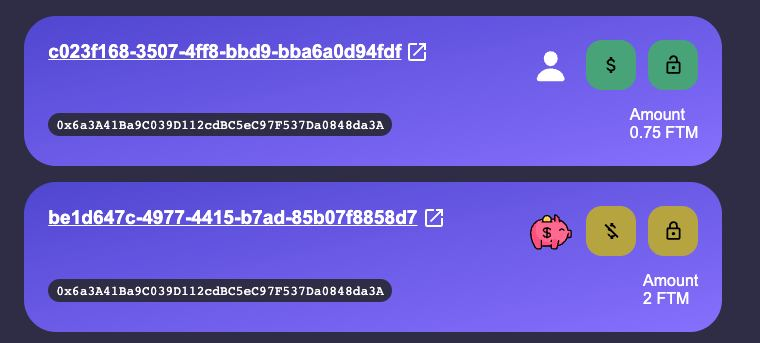
\includegraphics[scale=0.4]{immagini/Transaction/transactionsmall.jpg}
            \caption{Due esempi di transazione nella lista "Your Transactions"}
        \end{figure}
        \textbf{}\\
        In dettaglio, le transazioni presentano le proprie informazioni più importanti, quali:
        \begin{itemize}
            \item \textbf{Id del pagamento}: univoco, cliccabile, che rimanda alla pagina di riepilogo della transazione;
            \item \textbf{Indirizzo wallet acquirente} (o nel caso della MoneyBox, indirizzo del creatore della MoneyBox);
            \item \textbf{Icona che identifica il tipo del pagamento};
            \item \textbf{Icona che identifica lo stato del pagamento} (pagato, non pagato o rimborsato);
            \item \textbf{Icona che identifica lo stato del denaro} (bloccato o sbloccato);
            \item \textbf{Ammontare pagato} in Fantom\glo{} (FTM\glo{}).
        \end{itemize}
        Vediamo nel seguito come possono cambiare alcuni elementi:
            \subparagraph{Icona che identifica il tipo del pagamento}
            Può assumere due forme:
            \begin{itemize}
                \item \textbf{Pagamento singolo}
                \item \textbf{Pagamento MoneyBox}
            \end{itemize}
            \begin{figure}[H]
                \centering
                \begin{minipage}{0.45\textwidth}
                    \centering
                    
\includegraphics[scale=0.8]{immagini/Transaction/singleIcon.png} 
                    \caption{Icona pagamento singolo}
                \end{minipage}\hfill
                \begin{minipage}{0.45\textwidth}
                \centering
                    
\includegraphics[scale=0.8]{immagini/Transaction/MoneyBoxIcon.png} 
                    \caption{Icona pagamento MoneyBox}
                \end{minipage}
            \end{figure}
            \subparagraph{Icona che identifica lo stato del pagamento}
            Può assumere tre forme ben distinguibili dal colore:
            \begin{itemize}
                \item \textbf{Verde}: L'ordine si trova in stato "Paid";
                \item \textbf{Giallo}: L'ordine si trova in stato "Created";
                \item \textbf{Rosso}: L'ordine si trova in stato "Refunded"
            \end{itemize}
            \textbf{N.B.} \textit{Il giallo può apparire solo in ordini di tipo MoneyBox}
            \begin{figure}[H]
                \centering
                \begin{minipage}{0.33\textwidth}
                    \centering
                    
\includegraphics[scale=0.6]{immagini/Transaction/Paid.png} 
                    \caption{Stato: "Paid"}
                \end{minipage}\hfill
                \begin{minipage}{0.33\textwidth}
                \centering
                    
\includegraphics[scale=0.6]{immagini/Transaction/Created.png} 
                    \caption{Stato: "Created"}
                \end{minipage}
                \begin{minipage}{0.33\textwidth}
                    \centering
                        
\includegraphics[scale=0.6]{immagini/Transaction/Refunded.png} 
                        \caption{Stato: "Refunded"}
                    \end{minipage}
            \end{figure}
            \subparagraph{Icona che identifica lo stato del denaro}
            Può assumere due forme ben distinguibili dal colore:
            \begin{itemize}
                \item \textbf{Giallo}: L'ordine si trova in stato "Paid" o "Created". Il denaro si trova ancora all'interno dello smart contract\glo{};
                \item \textbf{Verde}: L'ordine si trova in stato "Unlocked". Il denaro è stato trasferito al wallet\glo{} del venditore.
            \end{itemize}
            \begin{figure}[H]
                \centering
                \begin{minipage}{0.45\textwidth}
                    \centering
                    
\includegraphics[scale=0.8]{immagini/Transaction/Locked.png} 
                    \caption{Stato: "Paid" o "Created"}
                \end{minipage}\hfill
                \begin{minipage}{0.45\textwidth}
                    \centering
                    
\includegraphics[scale=0.8]{immagini/Transaction/Unlocked.png} 
                    \caption{Stato: "Unlocked"}
                \end{minipage}
            \end{figure}